\documentclass[a4paper, 12pt]{article}%тип документа

%отступы
\usepackage[left=2cm,right=2cm,top=2cm,bottom=3cm,bindingoffset=0cm]{geometry}

%Русский язык
\usepackage[T2A]{fontenc} %кодировка
\usepackage[utf8]{inputenc} %кодировка исходного кода
\usepackage[english,russian]{babel} %локализация и переносы

%Вставка картинок
\usepackage{wrapfig}
\usepackage{graphicx}
\graphicspath{{pictures/}}
\DeclareGraphicsExtensions{.pdf,.png,.jpg}

%оглавление
\usepackage{titlesec}
\titlespacing{\chapter}{0pt}{-30pt}{12pt}
\titlespacing{\section}{\parindent}{5mm}{5mm}
\titlespacing{\subsection}{\parindent}{5mm}{5mm}
\usepackage{setspace}

%Графики
\usepackage{multirow}
\usepackage{pgfplots}
\pgfplotsset{compat=1.9}

%Математика
\usepackage{amsmath, amsfonts, amssymb, amsthm, mathtools}

%Заголовок
\author{Давыдов Владислав Олегович \\
Б04-005}
\title{\textbf{Работа 3.2.4\\Свободные колебания в электрическом контуре}}
\newtheorem{task}{Задача}
\date{}
\begin{document}
\maketitle
\newpage
\section*{Цель работы}
Исследование свободных колебаний в электрическом контуре.
\section*{В работе используются}
Генератор импульсов, электронное реле, магазин сопротивлений, магазин емкостей, катушка индуктивности, электронный осциллограф с разделительной панелью, измеритель LCR.
\section*{Теория}
\subsection*{Свободные колебания}
Рассмотрим электрический контур, состоящий из последовательно соединённых конденстора $C$, катушки индуктивности $L$ и резистора $R$. Обозначим разность потенциалов на конденсаторе $U_C$, а ток, текущий в контуре, через $I$. Второе првило Кирхгофа:
\begin{equation}
L \dfrac{d^2I}{dt^2}+R\dfrac{dI}{dt}+\dfrac{I}{C}=0.
\end{equation}
Вводя обозначения $\gamma = \dfrac{R}{2L}$, $\omega_0^2=\dfrac{1}{LC}$, получим уравнение
\begin{equation}
\ddot{I}+2\gamma\dot{I}+\omega_0^2I=0.
\end{equation}
Его решение в общем виде:
\begin{equation}
I = -\dfrac{U_0}{L\kappa}e^{-\gamma t}\text{sh}(\kappa t), 
\end{equation}
где $\kappa = \sqrt{\gamma^2 - \omega_0^2}$, $U_0 = U_C$ -- начальное напряжение на конденсаторе.
\begin{equation}
T_{0} = \dfrac{1}{\nu}, \; T = T_{0} \dfrac{x}{n x_{0}} , \; \nu_{0} = \dfrac{1}{2 \pi \sqrt{L C}} = 5 \; kHz ,
\end{equation}
\begin{equation}
R_{kr} = 2 \sqrt{\dfrac{L}{C}} ,
\end{equation}
\begin{equation}
\theta = \dfrac{1}{n} ln \dfrac{U_{k}}{U_{k+n}} ,
\end{equation}
\newpage
\section*{Экспериментальная установка}
\section*{Установка}
\begin{figure}[h!]
\begin{center}
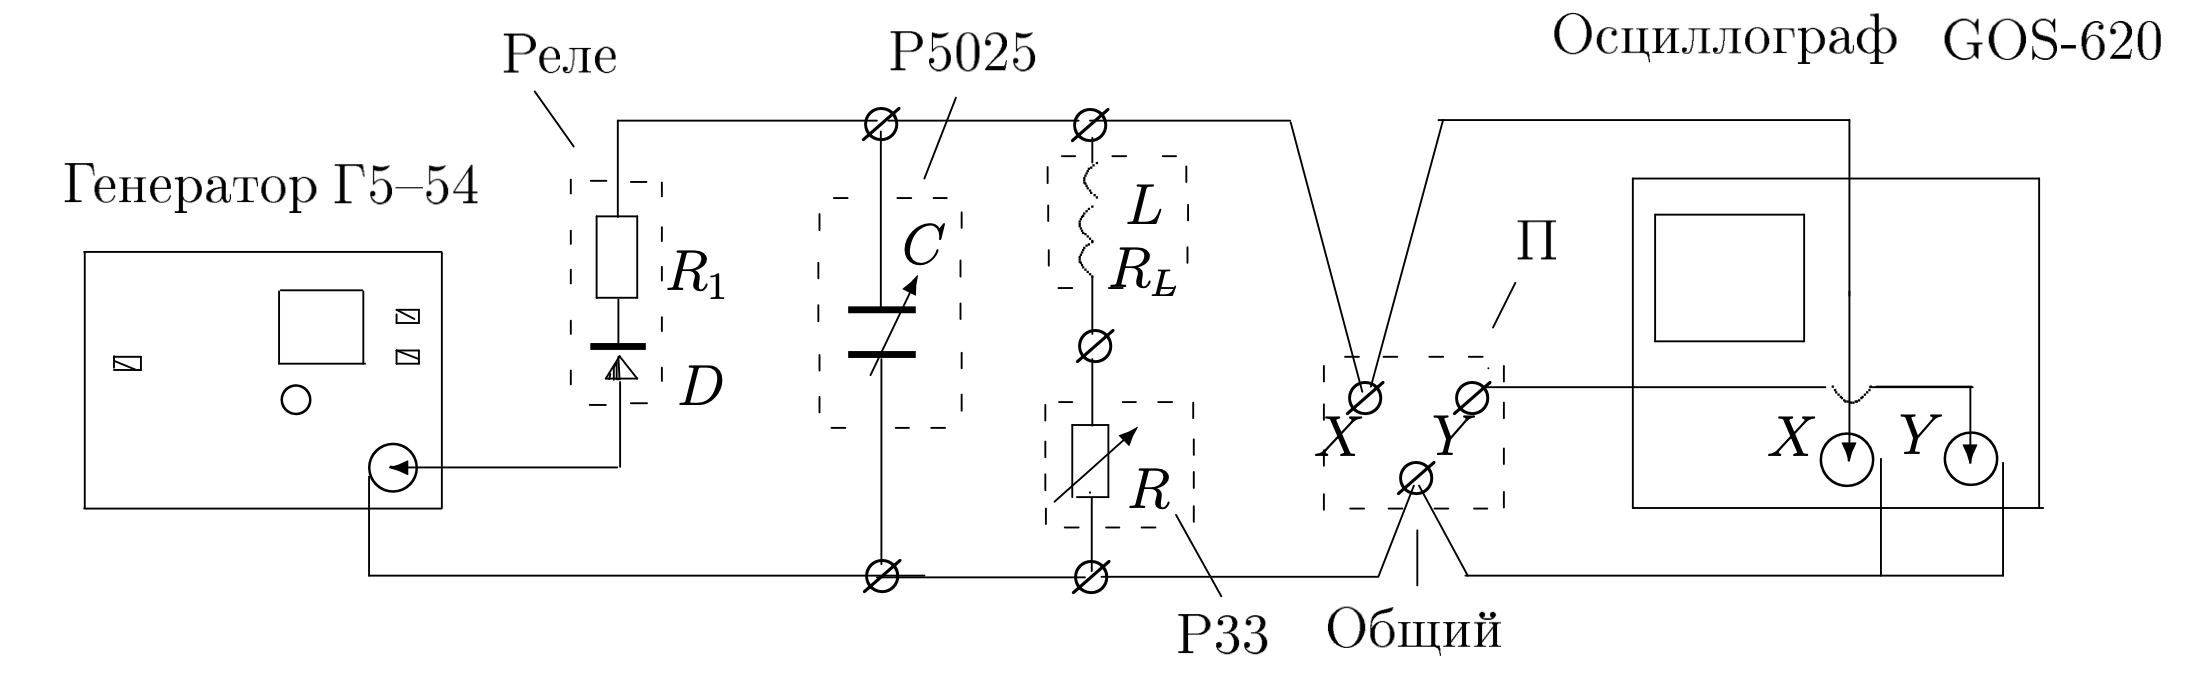
\includegraphics[width = 0.9\textwidth]{1.png}
\caption{Схема установки}
\end{center}
\end{figure}

\section*{Ход работы}
Измерим период в зависимости от емкости конденсатора

\begin{table}[h!]
\begin{center}

\begin{tabular}{|c|c|c|}
\hline
$T$, мс & $C$, мкФ  \\ \hline
1,2        & 0,02       \\ \hline
1,25      & 0,10      \\ \hline
1,67      & 0,18      \\ \hline
2,00 & 0,26 \\ \hline
2,30 & 0,34 \\ \hline
2,53 & 0,42 \\ \hline
2,80 & 0,50 \\ \hline
3,00 & 0,58 \\ \hline
3,20 & 0,66 \\ \hline
3,40 & 0,74 \\ \hline
3,60 & 0,82 \\ \hline
3,80 & 0,90 \\ \hline

\end{tabular}
\caption{Период свободных колебаний от емкости конденсатора.}
\end{center}
\end{table}

\newpage
\subsection*{Критическое сопротивление и декремент затухания.}
Приняв $ L = 200 $ мГн, рассчитаем емкость при которой собственная частота контура составляет 5 кГц
\begin{center}
$ C = (\dfrac{1}{2 \pi \nu_{0}})^{2} \dfrac{1}{L} = 5 * 10^{-9} $ Ф, $ R_{kr} = 12650$ Ом.
\end{center}



\begin{table}[h!]
\begin{center}

\begin{tabular}{|c|c|c|}
\hline
$R$, кОм & $n$, & $\theta$   \\ \hline
1,3        & 2 &  1,3    \\ \hline
1,7      & 2  &  0,70  \\ \hline
2,1      & 2    & 0,83 \\ \hline
2,5 & 1 & 1,10 \\ \hline
2,9 & 1 & 1,16 \\ \hline
3,3 & 1 & 1,18 \\ \hline
2,1 & 1 & 0,85 \\ \hline
1,7 & 1 & 0,69 \\ \hline

\end{tabular}
\caption{Декремент затухания от сопротивления.}
\end{center}
\end{table}

\newpage
\subsection*{Свободные колебания на фазовой плоскости.}
\begin{center}
Выставив на осциллографе в канал Y напряжение $U_{R} \sim I \sim \dfrac{dU_{C}}{dt}$, получим следующие осциллограммы:
\begin{figure}[h!]
\begin{center}
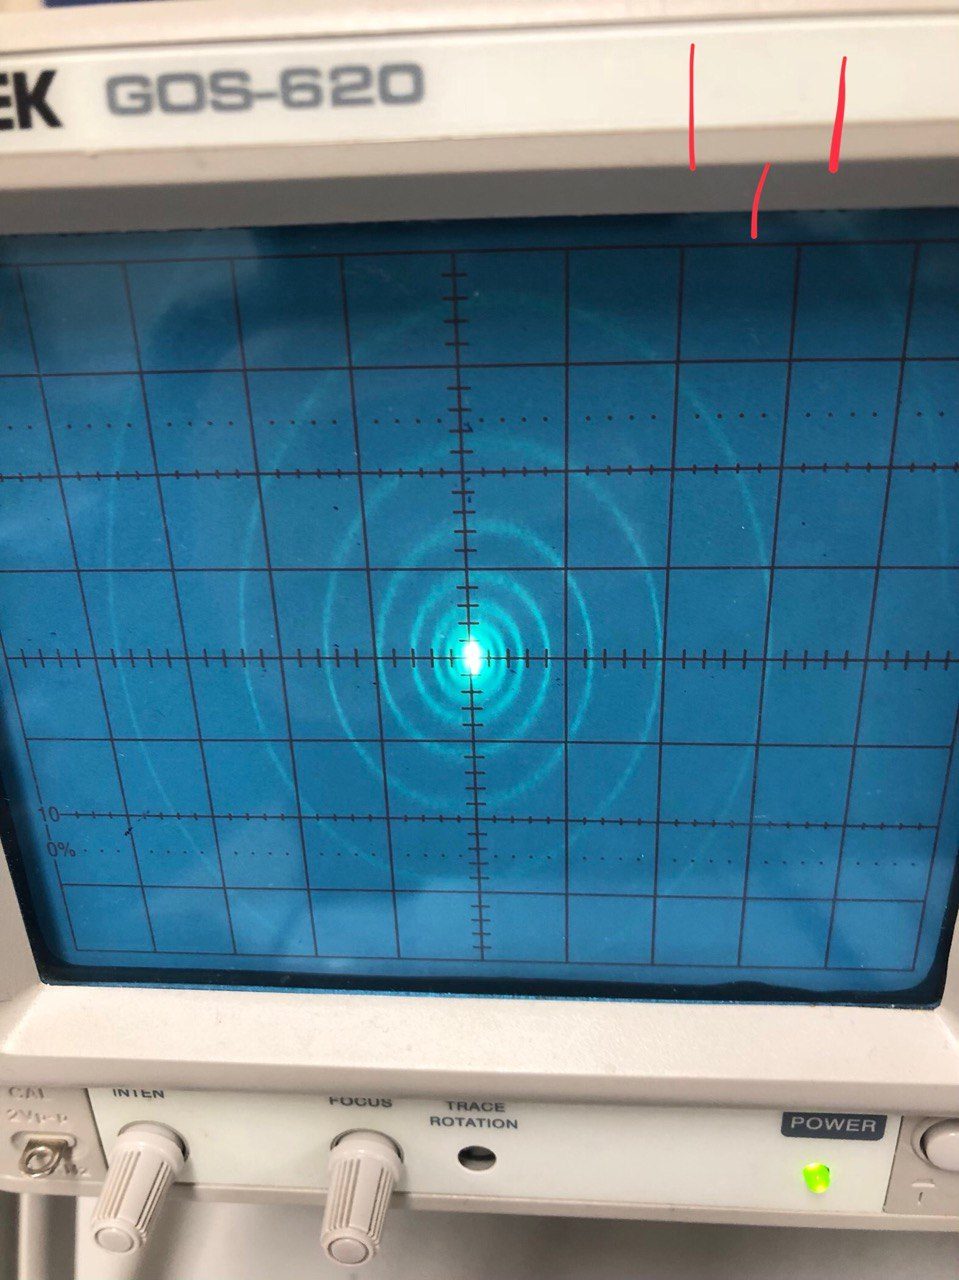
\includegraphics[width = 0.34\textwidth]{11.jpeg}
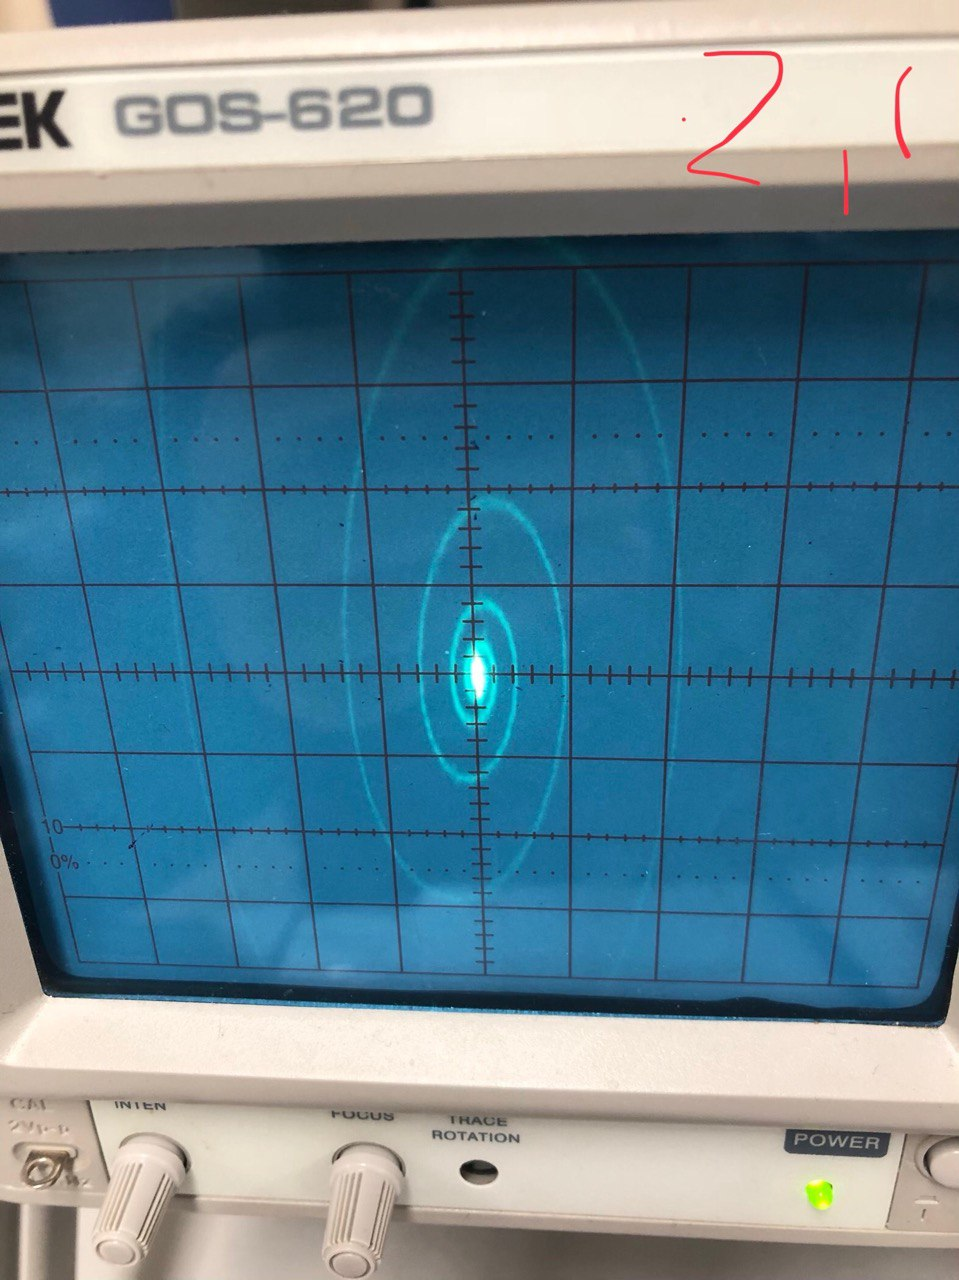
\includegraphics[width = 0.34\textwidth]{21.jpeg}
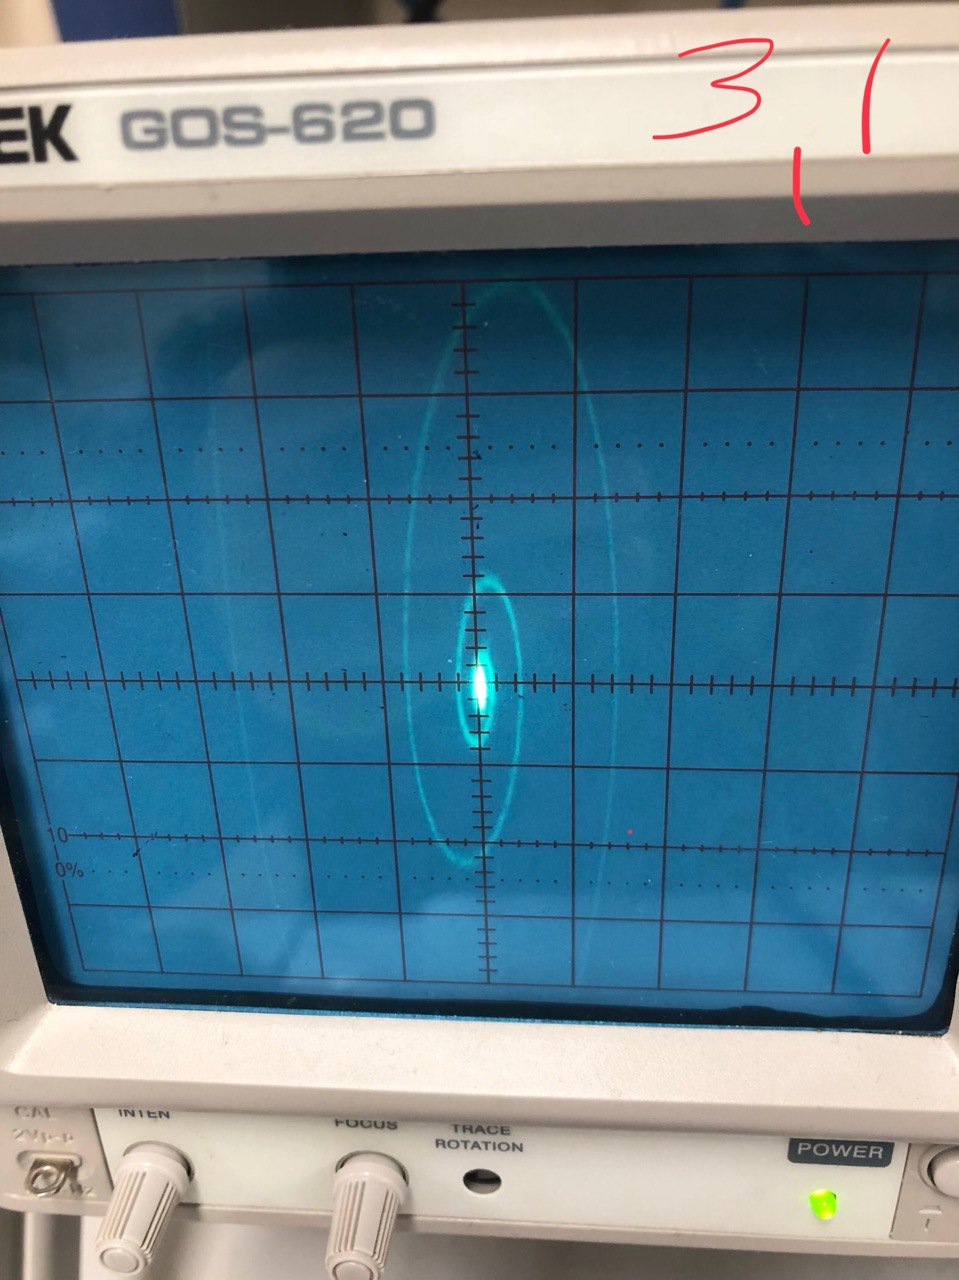
\includegraphics[width = 0.34\textwidth]{31.jpeg}
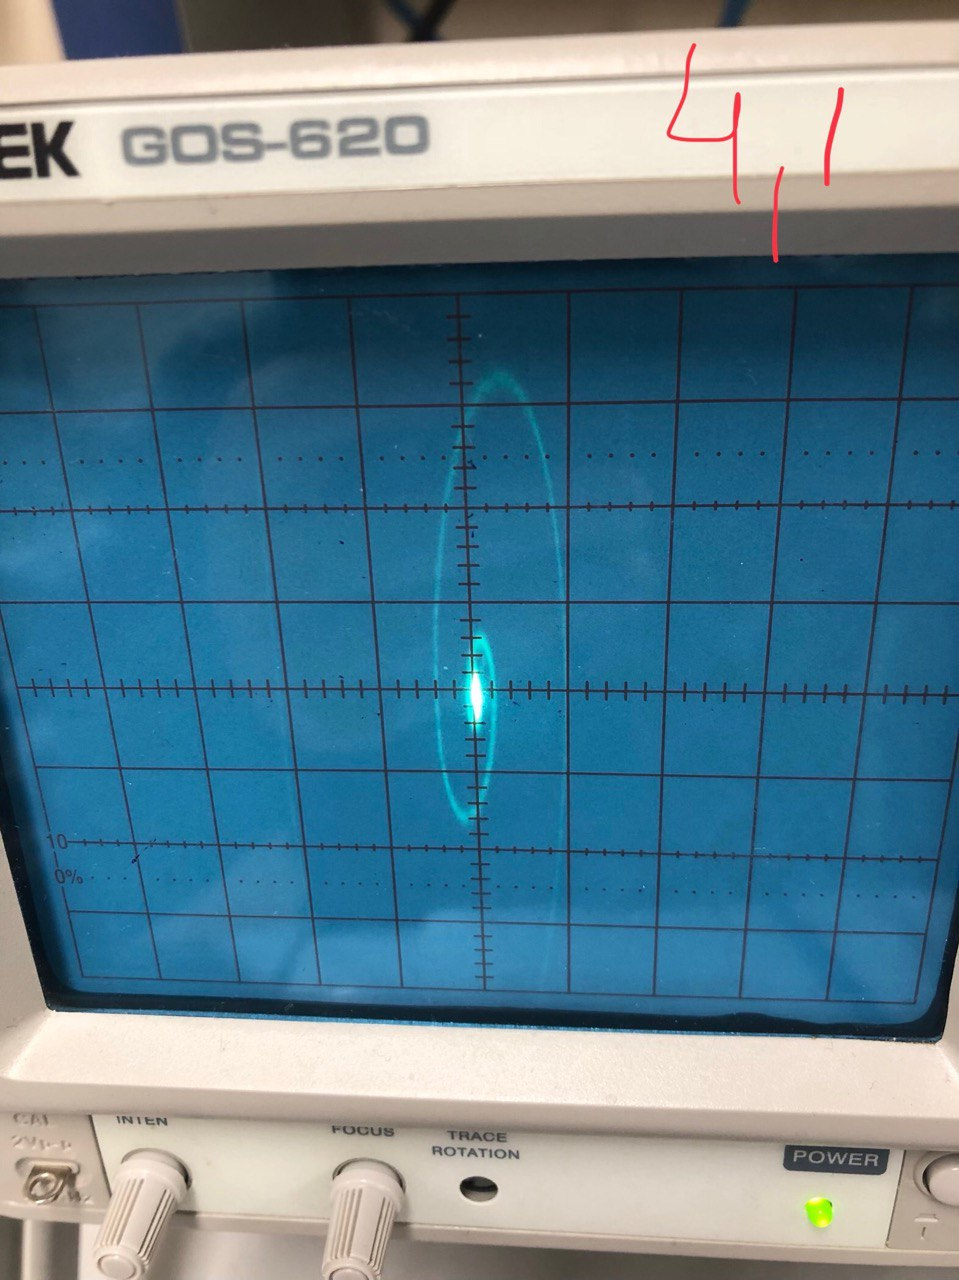
\includegraphics[width = 0.34\textwidth]{41.jpeg}
\end{center}
\end{figure}
\end{center}


\begin{center}
Далее, измерим параметры катушки, с помощью измерителя LCR:

\begin{table}[h!]
\begin{center}
\begin{tabular}{|c|c|c|}
\hline
$\nu$ & $R$, Ом & $L$, мГн   \\ \hline
1 кГц       & 24,0 &  385,2    \\ \hline
5 кГц      & 42,5  &  387,0  \\ \hline
50 Гц      & 15,3    & 394,7 \\ \hline

\end{tabular}
\caption{Параметры катушки при разной частоте.}
\end{center}
\end{table}
Сопротивление катушки при постоянном токе = 14 Ом.

\end{center}
\newpage
\subsection*{Обработка результатов.}
\begin{center}
$T_{teor}$ будем вычислять по формуле:
\begin{equation}
T_{teor} = 2 \pi \sqrt{L C}
\end{equation}
\begin{figure}[h!]
\begin{center}
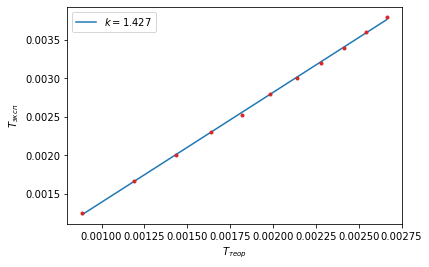
\includegraphics[width = 0.8\textwidth]{2.png}
\caption{Зависимость экспериментально вычисленного периода от теоретического}
\end{center}
\end{figure}
\\
Их расхождение может значить другое значение индуктивности катушки (в нашем примере мы предполагали индуктивность катушки равную примерно 200мГн). \\
\end{center}

\newpage
\begin{center}
Вычислим критическое сопротивление по следующей формуле:
\begin{equation}
R_{kr} = 2 \pi \sqrt{\Delta Y / \Delta X}
\end{equation}

\begin{figure}[h!]
\begin{center}
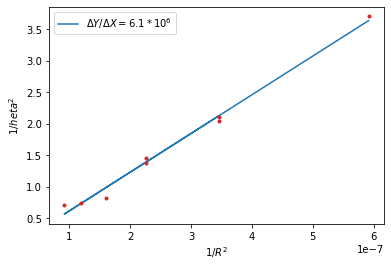
\includegraphics[width = 0.8\textwidth]{3.png}
\caption{Зависимость Y от X}
\end{center}
\end{figure}
Получаем значение для $R_{kr} = 15,5$ кОм, что приблизительно совпадает с нашим первоначальным результатом ($R_{kr} = 12,7$ кОм).


\begin{table}[h!]
\begin{center}
\begin{tabular}{|c|c|c|c|c|c|c|c|}
\hline
$L_{kat}$, мГн & $R_{kr}$ теор, кОм & $R_{kr}$ график, кОм & & $R$, кОм  & $Q$ теор &  $Q f(\theta)$  \\ \hline
387       & 12,7  & 15,5 & & min =  & 2,7 & 6,3    \\ \hline
387     & 12,7  & 15,5 & & max = & 6,0 & 16,0  \\ \hline

\end{tabular}
\caption{Результаты.}
\end{center}
\end{table}
\end{center}


\end{document}